% ============================================================
\section{Introduction}
\label{sec:introduction}
% ============================================================

Electric vehicles (EVs) connected through bidirectional chargers can
return energy to the grid and adjust their charging power within
seconds. This vehicle-to-grid (V2G) capability allows an aggregated
fleet to take part in services that were traditionally supplied by
synchronous plant and network assets \cite{Kempton2005}. Two of these
services are of direct interest to network operators. At the
distribution level, the active power of a fleet changes feeder flows
and can therefore relieve undervoltage at heavily loaded hours or absorb
surplus photovoltaic (PV) output that would otherwise raise voltages
above the statutory band \cite{AmamraMarco2019,HuEtAl2022,AnEtAl2024}.
At the bulk-system level, fast converter control lets the same fleet
respond to frequency deviations and support primary and secondary
frequency control \cite{Lam2016,Izadkhast2015}. The two services draw
on the same converter rating and the same stored energy. A fleet that
discharges at its full rating to lift an evening voltage profile has no
headroom left for upward frequency response, and a fleet that has been
emptied in the evening must be recharged before the next departure.
The way the available capability is divided between the two services
is therefore a scheduling decision in its own right.

The coupling is becoming more relevant as converter-interfaced
generation displaces synchronous machines. Lower inertia raises the
rate of change of frequency and deepens the frequency nadir after a
disturbance, so the value of fast reserve varies over the day with the
PV share \cite{Tielens2016}. The same midday hours often coincide with
reverse power flow and overvoltage on PV-rich feeders, whereas the
evening peak produces undervoltage on residential feeders while PV is
absent. A controller that coordinates voltage support and frequency
reserve must therefore act on two very different time scales: hourly
energy decisions that respect network voltage limits and fleet energy,
and second-level frequency dynamics that depend on how much reserve has
been withheld.

The literature addresses these services largely in isolation. Studies
on V2G voltage regulation solve power flow on distribution test feeders
and use model predictive or robust control of charger active or
reactive power \cite{AmamraMarco2019,HuEtAl2022,AnEtAl2024,YuanEtAl2026}.
Reinforcement learning (RL) has been applied to two-time-scale voltage
control in active distribution systems \cite{Cao2022}, but frequency
dynamics are outside the scope of those formulations. Conversely, RL
methods for load-frequency control (LFC) train agents on multi-area
dynamic models with tie lines and area control error (ACE)
\cite{YanXu2020,Abouheaf2019,MaHuSong2024,ZhaoLiuHill2025,Wu2024Symmetry}.
Several studies use V2G as the regulating resource
\cite{Alfaverh2023,Liang2026Symmetry,Xiong2026Symmetry}, and an
actor--critic PPO scheme has been used to mitigate EV-based
load-altering attacks on microgrid LFC \cite{AbazariEtAl2025}.
In these frequency-oriented formulations the fleet enters the
frequency model as an aggregate power source, and the feeder voltages
that result from the scheduled fleet power are not part of the
evaluation. Aggregate
PEV models for primary frequency control have been extended with
distribution losses and current limits \cite{Izadkhast2015,Izadkhast2016},
yet the allocation of fleet capability between voltage support and
frequency reserve is fixed in advance rather than optimized. Planning
and stability studies on EV charging infrastructure in Thai networks
\cite{YenchamchalitEtAl2018PSO,YenchamchalitEtAl2021LFO,Yenchamchalit2021,
Kongjeen2019,Nuamkoksung2025} address siting, sizing, and oscillatory
stability, which are complementary to operational coordination.

This paper addresses that gap with a two-time-scale formulation in
which an RL agent decides, for each area and each hour, both the V2G
active-power set-point and the share of the plugged-in converter
rating that is withheld as frequency-regulation reserve. The decision
is evaluated on two physically specified layers. The slow layer solves
an AC power flow on an IEEE 33-bus feeder \cite{BaranWu1989} in each
area and updates an energy-consistent fleet model. The fast layer
simulates a two-area LFC system with inertia, damping,
governor-turbine dynamics, a tie line with a synchronizing coefficient,
ACE-based automatic generation control (AGC), and a saturated V2G droop
loop whose gain and limit follow from the reserve decision. The agent
is trained with proximal policy optimization (PPO) \cite{Schulman2017}
and evaluated against independently simulated benchmark controllers.

The contributions are as follows.
\begin{itemize}
\item A two-time-scale V2G environment that couples branch-resolved AC
power flow on two IEEE 33-bus feeders with a dynamic two-area LFC model
in physical units. Fleet size, charger rating, battery capacity,
charging and discharging efficiencies, plug-in availability, driving
energy, and tie-line dynamics are specified explicitly. The power-flow
solver and the LFC model are verified against pandapower
\cite{Thurner2018} and against closed-form steady-state values.

\item A joint action formulation in which each area aggregator selects
an hourly set-point and a reserve share. The reserve share sets the
droop gain and saturation of the fleet in the LFC layer, which exposes
the trade-off between voltage support and frequency reserve under
state-of-charge (SoC), availability, and time-varying inertia
constraints. The reward penalizes both undervoltage and overvoltage,
frequency nadir, tie-line deviation, battery throughput, and terminal
SoC deficit.

\item A reproducible learning and evaluation protocol. PPO is trained
with five independent seeds on randomized load, PV, fleet
participation, and disturbance scenarios. The learned policies are
evaluated on 30 held-out days and 20 out-of-distribution stress days
against uncontrolled charging, a conventional rule-based volt-watt and
droop controller, and a day-ahead optimization with perfect foresight.
A reward ablation quantifies the effect of each penalty term. Code and
data are released with the paper.
\end{itemize}

The remainder of the paper is organized as follows.
Section~\ref{sec:model} presents the system model.
Section~\ref{sec:control} formulates the control problem, the PPO
training procedure, and the benchmark controllers.
Section~\ref{sec:results} reports the results, and
Section~\ref{sec:conclusions} concludes the paper.

% ============================================================
\section{System Model}
\label{sec:model}
% ============================================================

\subsection{Overview and Time Scales}

Fig.~\ref{fig:architecture} summarizes the framework. Two
interconnected control areas each contain a population of
distribution feeders hosting PV units and an aggregated V2G fleet. Each
area's distribution system is represented by $N_f=25$ identical copies
of a representative IEEE 33-bus feeder, so that the area-level fleet
power and reserve are $N_f$ times the per-feeder values while the
voltage response is evaluated on the representative feeder. The slow
layer advances in hourly steps over a 24-h horizon. The fast layer
simulates a 60-s window of frequency dynamics at a 20-ms integration
step for every hour, using the reserve that the slow layer has made
available. The episode starts at 12:00 and ends at 12:00 on the
following day so that the evening discharge and the overnight recharge
fall inside one episode.

\begin{figure*}[!t]
\centering
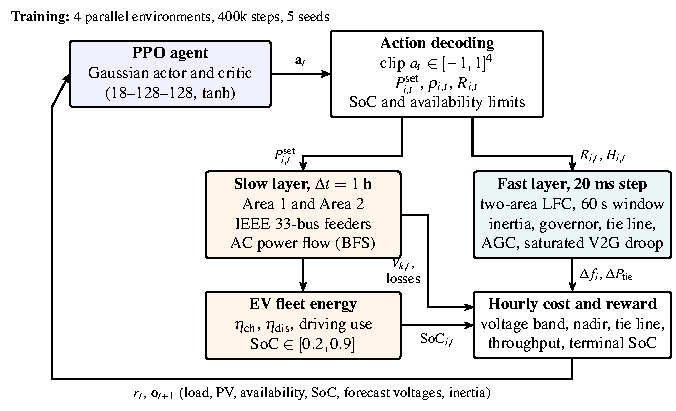
\includegraphics[width=0.78\textwidth]{fig_architecture.pdf}
\caption{Two-time-scale V2G coordination framework. The PPO agent sets
the hourly V2G set-point and the frequency-reserve share of each area.
The slow layer solves AC power flow on the IEEE 33-bus feeder of each
area and updates fleet energy; the fast layer simulates two-area LFC
dynamics with the reserve-dependent V2G droop.}
\label{fig:architecture}
\end{figure*}

\subsection{Distribution Feeders}
\label{sec:feeders}

Both areas use the branch impedances and nominal loads of the IEEE
33-bus system \cite{BaranWu1989} at 12.66~kV, taken from the pandapower
case library \cite{Thurner2018}. The five normally open tie switches are
kept open so that the feeder remains radial. The net load at bus $k$
of area $i$ in hour $t$ is
\begin{equation}
P_{k,t} = \lambda_{i,t}P_k^{0}-P^{\mathrm{PV}}_{k,t}-P^{\mathrm{EV}}_{k,t},
\qquad
Q_{k,t} = \lambda_{i,t}Q_k^{0},
\label{eq:netload}
\end{equation}
where $P_k^{0}$ and $Q_k^{0}$ are the nominal loads, $\lambda_{i,t}$ is
the normalized load profile, and positive $P^{\mathrm{EV}}_{k,t}$
denotes discharge. The fleet set-point is shared equally among the V2G
hubs of the area, and the PV output is shared equally among the PV
buses (Fig.~\ref{fig:feeder}). Area~1 is a residential feeder with
1.5~MW of PV and hubs in the downstream half of the main feeder
(buses 13, 17, and 18) and at the end of the bus 26 to 33 lateral. Area~2 is a mixed commercial and residential feeder
with 4.2~MW of PV concentrated at the feeder ends, which produces
midday overvoltage when PV output is high.

The power flow is solved by the direct backward/forward sweep of
\cite{Teng2003}. With the bus-injection to branch-current matrix
$\mathbf{B}$ and the branch impedance vector $\mathbf{z}$, the bus
voltages are updated as
\begin{equation}
\mathbf{V}^{(m+1)} = V_0\mathbf{1}-\mathbf{B}^{T}\operatorname{diag}(\mathbf{z})\mathbf{B}\,
\overline{\left(\mathbf{S}\oslash\mathbf{V}^{(m)}\right)},
\label{eq:bfs}
\end{equation}
until the largest voltage update falls below $10^{-9}$~p.u., where
$\mathbf{S}$ is the complex net load vector and $\oslash$ denotes
element-wise division. The active-power loss is
$\sum_{b}r_b|I_b|^{2}$ over all branches $b$.

\begin{figure*}[!t]
\centering
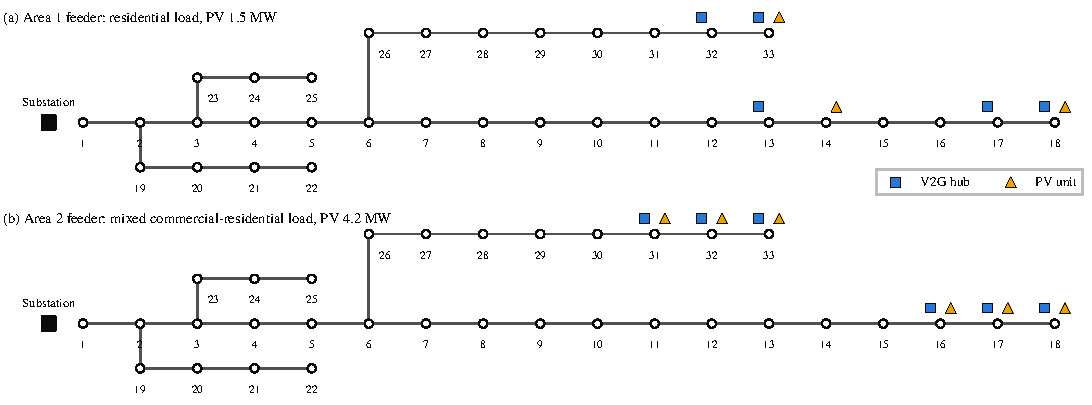
\includegraphics[width=\textwidth]{fig_feeder.pdf}
\caption{IEEE 33-bus feeders used in the two areas, with V2G hubs and
PV units. The topology and impedances are those of \cite{BaranWu1989}.}
\label{fig:feeder}
\end{figure*}

\subsection{Daily Profiles and Scenario Generation}
\label{sec:profiles}

Fig.~\ref{fig:profiles} shows the nominal daily profiles. The
residential profile has a morning shoulder and an evening peak at
19:00 to 21:00, and the mixed profile has a broad daytime plateau and an
evening peak. Both profiles are synthetic; their shapes follow the
measured residential and commercial low-voltage consumer curves of
\cite{Jardini2000}, with a residential evening peak and a commercial
daytime plateau, and are normalized to a peak of 1.0. The PV profile
follows a clear-sky shape between 06:00 and 18:00. Area~1 represents
home charging, with about 90\% of the fleet plugged in at night and 30\%
during working hours, which reproduces the pattern of residential
charging availability observed in the EV Project, low during the day
and high overnight \cite{Schey2012}. Area~2 represents workplace
charging with the opposite pattern, following the observation that
vehicles with access to workplace charging are typically parked there
for 4 to 10 h on working days \cite{INL2014}.

Each training or evaluation day is drawn from a scenario generator that
scales the area load by a factor in $[0.85,1.10]$, applies a cloud
factor in $[0.3,1.0]$ with hour-to-hour PV variability, scales fleet
participation by a factor in $[0.7,1.1]$, adds 3\% multiplicative noise
to the hourly load, and draws the initial SoC in $[0.50,0.60]$. Stress
days use heavier load ($[1.10,1.20]$), lower fleet participation
($[0.55,0.70]$), and disturbances 1.3 to 1.6 times larger, all outside
the training ranges, together with near clear-sky PV ($[0.9,1.0]$),
which lies at the upper end of the training range. Stress days are
never seen during training.

\begin{figure}[!t]
\centering
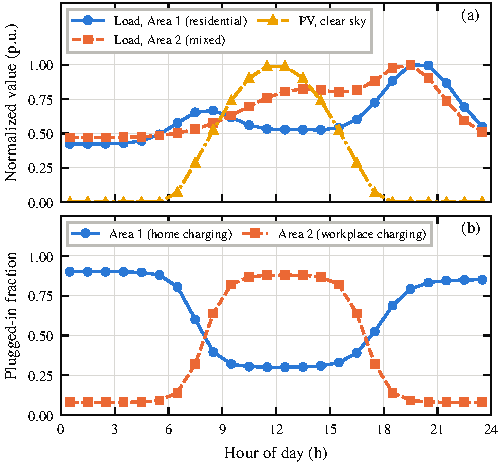
\includegraphics[width=\columnwidth]{fig_profiles.pdf}
\caption{Nominal daily profiles. (a) Normalized load of each area and
clear-sky PV. (b) Fraction of the fleet plugged in.}
\label{fig:profiles}
\end{figure}

\subsection{Aggregated EV Fleet}
\label{sec:fleet}

Each representative feeder hosts $N_{\mathrm{EV}}=300$ vehicles with
60-kWh batteries and 7.4-kW bidirectional chargers. The usable SoC
range is 0.20 to 0.90, and the charging and discharging efficiencies
are $\eta_{\mathrm{ch}}=\eta_{\mathrm{dis}}=0.92$. Each vehicle uses
9~kWh per day for driving, which corresponds to about 45~km at a
real-driving consumption of about 190~Wh/km; more than 80\% of European
drivers cover less than 65~km per day and the median real-driving
consumption of a small battery electric car was 186~Wh/km in the Green
eMotion field data \cite{Donati2015}. The driving energy is distributed
over the hours in which the vehicle is away in proportion to the
unplugged fraction. The fleet is
treated as one aggregated battery with energy capacity
$E^{\mathrm{cap}}=18$~MWh per feeder. The plugged-in rating is
\begin{equation}
P^{\mathrm{rate}}_{i,t}=\chi_{i,t}\,\kappa_i\,N_{\mathrm{EV}}\,P_{\mathrm{ch}},
\label{eq:prate}
\end{equation}
where $\chi_{i,t}$ is the plugged-in fraction and $\kappa_i$ the
participation factor of the scenario. With the driving energy
$E^{\mathrm{drv}}_{i,t}$ deducted first, the energy-feasible limits
for $\Delta t=1$~h are
\begin{align}
\bar P^{\mathrm{dis}}_{i,t}&=\min\!\left\{P^{\mathrm{rate}}_{i,t},\,
\eta_{\mathrm{dis}}\frac{E_{i,t}-E^{\mathrm{drv}}_{i,t}-E^{\min}}{\Delta t}\right\}^{+},
\label{eq:pdis}\\
\bar P^{\mathrm{ch}}_{i,t}&=\min\!\left\{P^{\mathrm{rate}}_{i,t},\,
\frac{E^{\max}-E_{i,t}+E^{\mathrm{drv}}_{i,t}}{\eta_{\mathrm{ch}}\Delta t}\right\}^{+},
\label{eq:pch}
\end{align}
and the energy is updated as
\begin{equation}
E_{i,t+1}=E_{i,t}-\frac{P^{\mathrm{dis}}_{i,t}\Delta t}{\eta_{\mathrm{dis}}}
+\eta_{\mathrm{ch}}P^{\mathrm{ch}}_{i,t}\Delta t-E^{\mathrm{drv}}_{i,t}
+\Delta E^{\mathrm{reg}}_{i,t},
\label{eq:energy}
\end{equation}
with $P^{\mathrm{dis}}=\max(P^{\mathrm{set}},0)$ and
$P^{\mathrm{ch}}=\max(-P^{\mathrm{set}},0)$. If driving alone would take
the energy below $E^{\min}$, the shortfall is recorded as unmet
mobility energy and penalized.

The last term of \eqref{eq:energy} is the battery energy exchanged by
the frequency droop loop of Section~\ref{sec:lfcmodel}. The fast layer
simulates a window of length $\tau_w=60$~s in every hour, which is
too short to integrate the energy of a full hour directly. Four
treatments of this term are compared in Section~\ref{sec:regenergy}.
Let $E^{\mathrm{out}}$ and $E^{\mathrm{in}}$ denote the energy
delivered to and absorbed from the grid by the area droop power over a
simulated interval, $E^{\mathrm{out}}=\int\max(\Delta P_{\mathrm{ev},i},0)\,d\tau$
and $E^{\mathrm{in}}=\int\max(-\Delta P_{\mathrm{ev},i},0)\,d\tau$. The
battery-side energy per feeder is
\begin{equation}
\Delta E^{\mathrm{reg}}_{i,t}=\frac{1}{N_f}\left(
-\frac{E^{\mathrm{out}}_{i,t}}{\eta_{\mathrm{dis}}}+\eta_{\mathrm{ch}}E^{\mathrm{in}}_{i,t}\right),
\label{eq:regenergy}
\end{equation}
so that every round trip is lossy. The treatments differ in how
$E^{\mathrm{out}}$ and $E^{\mathrm{in}}$ are obtained for the hour:
(i) \emph{none}, the term is neglected (the model of the first
submission, used for diagnosis only); (ii) \emph{window}, only the
simulated 60~s are counted; (iii) \emph{hourly extrapolation}, the
window energy is multiplied by $3600/\tau_w=60$, which implicitly
assumes that the step disturbance of the window recurs every minute;
(iv) \emph{decomposed}, the window containing the step event is counted
once and a second 60-s simulation of the same hour with the
fluctuating component only is scaled to the remaining 59~min,
\begin{equation}
E^{\mathrm{out}}_{i,t}=E^{\mathrm{out}}_{\mathrm{step+fluct}}
+\left(\frac{3600}{\tau_w}-1\right)E^{\mathrm{out}}_{\mathrm{fluct}},
\label{eq:decomposed}
\end{equation}
and likewise for $E^{\mathrm{in}}$. Treatment (iv) is the default of the
environment used for training and for all reported results. Its
accuracy is checked against an exact 3600-s simulation of the fast
layer for every hour of the evaluation (Section~\ref{sec:regenergy}),
which is too slow to use during training.

\subsection{Two-Area Load-Frequency Control Model}
\label{sec:lfcmodel}

The fast layer uses the standard linearized two-area LFC model
\cite{Kundur1994,Bevrani2014} with non-reheat turbines, extended with a
V2G droop loop in each area \cite{Izadkhast2015}. In per unit on the
area base $P_r=500$~MW and with frequency deviation $\Delta f_i$ in per
unit of $f_0=50$~Hz,
\begin{align}
2H_{i,t}\,\dot{\Delta f_i}&=\Delta P_{m,i}+\Delta P_{\mathrm{ev},i}-\Delta P_{L,i}
-a_i\Delta P_{\mathrm{tie}}-D_i\Delta f_i,\label{eq:swing}\\
T_{g,i}\,\dot{\Delta P_{g,i}}&=\Delta P_{c,i}-\Delta f_i/R_i-\Delta P_{g,i},\\
T_{t,i}\,\dot{\Delta P_{m,i}}&=\Delta P_{g,i}-\Delta P_{m,i},\\
\dot{\Delta P_{\mathrm{tie}}}&=2\pi f_0T_{12}\,(\Delta f_1-\Delta f_2),\\
\mathrm{ACE}_i&=B_i\Delta f_i+a_i\Delta P_{\mathrm{tie}},\quad
\Delta P_{c,i}=-K_I\!\int\!\mathrm{ACE}_i\,dt,\label{eq:ace}\\
T_{\mathrm{ev}}\,\dot{\Delta P_{\mathrm{ev},i}}&=
\operatorname{sat}_{\pm r_{i,t}}\!\left(-K_{\mathrm{ev},i,t}\Delta f_i\right)-\Delta P_{\mathrm{ev},i},
\label{eq:evdroop}
\end{align}
where $a_1=1$, $a_2=-1$, $B_i=1/R_i+D_i$, and $r_{i,t}=N_fR_{i,t}/P_r$
is the area V2G reserve in per unit. The droop gain is
$K_{\mathrm{ev},i,t}=r_{i,t}f_0/\Delta f_{\mathrm{full}}$, so the full
reserve is deployed at $\Delta f_{\mathrm{full}}=0.2$~Hz and the
response saturates beyond that point. The first-order lag
$T_{\mathrm{ev}}=0.15$~s represents aggregator communication and
converter response. Aggregated EV fleets are commonly represented in
LFC studies by a first-order transfer function with time constants
between 0.1 and 1~s \cite{KoSung2018,Ziras2017}; the chosen value lies
at the fast end of this range; the settling time of about 1~s
measured for charger response to local frequency measurements and
reported in \cite{Ziras2017} corresponds to roughly three to five such
time constants.

Inertia falls when PV displaces synchronous generation. The hourly
inertia constant is
\begin{equation}
H_{i,t}=H_i^{0}\left(1-\gamma_i S_{i,t}\right),
\label{eq:inertia}
\end{equation}
where $S_{i,t}$ is the normalized PV output and $\gamma_1=0.20$,
$\gamma_2=0.35$ reflect the higher PV share of Area~2
\cite{Tielens2016}. In each hour the window contains a step load change
at $t=2$~s in one randomly selected area, with magnitude
$0.03\,\delta\,u$~p.u., where $\delta$ is the scenario disturbance scale
and $u$ is uniform in $[0.5,1.0]$ with a random sign, plus an
Ornstein--Uhlenbeck fluctuation with a 10-s time constant and standard
deviation $0.006\,(0.3+2S_{i,t}(1.2-c_i))$~p.u., where $c_i$ is the
cloud factor, so that the fluctuation grows with PV output under
partial cloud. The disturbance of
each hour is generated from a seed fixed by the scenario and the hour,
so every controller faces identical disturbances. Equations
\eqref{eq:swing} to \eqref{eq:evdroop} are integrated with the
fourth-order Runge--Kutta method. Table~\ref{tab:params} lists all
parameters.

\begin{table}[!t]
\caption{Model, fleet, and training parameters.}
\label{tab:params}
\centering
\footnotesize
\setlength{\tabcolsep}{3pt}
\begin{tabular}{p{0.60\columnwidth}p{0.34\columnwidth}}
\toprule
\textbf{Parameter} & \textbf{Value}\\
\midrule
\multicolumn{2}{l}{\emph{Feeder and fleet (per representative feeder)}}\\
Feeder / base voltage & IEEE 33-bus / 12.66 kV\\
PV rating, Area 1 / Area 2 & 1.5 / 4.2 MW\\
EVs, battery, charger & 300, 60 kWh, 7.4 kW\\
SoC limits; $\eta_{\mathrm{ch}}=\eta_{\mathrm{dis}}$ & 0.20 to 0.90; 0.92\\
Driving energy per EV & 9 kWh/day\\
Feeders per area $N_f$ & 25\\
\multicolumn{2}{l}{\emph{Two-area LFC}}\\
Area base $P_r$; $f_0$ & 500 MW; 50 Hz\\
$H_1^0$, $H_2^0$; $\gamma_1$, $\gamma_2$ & 5.0, 4.0 s; 0.20, 0.35\\
$D_i$; $R_i$ & 1.0 p.u.; 0.05 p.u.\\
$T_{g,1}$, $T_{g,2}$; $T_{t,1}$, $T_{t,2}$ & 0.08, 0.10 s; 0.40, 0.45 s\\
$T_{12}$; $K_I$ & 0.08 p.u./rad; 0.05\\
$T_{\mathrm{ev}}$; $\Delta f_{\mathrm{full}}$ & 0.15 s; 0.2 Hz\\
Window; integration step & 60 s; 20 ms (RK4)\\
Load step; OU base std. & 0.03$\delta u$; 0.006 p.u.\\
\multicolumn{2}{l}{\emph{Control and reward}}\\
Voltage band & 0.95 to 1.05 p.u.\\
$\rho_{\max}$ & 0.6\\
$w_V$, $w_f$, $w_{\mathrm{tie}}$, $w_{\mathrm{deg}}$, $w_E$, $w_U$ & 50, 4, 0.5, 0.05, 1, 100\\
\multicolumn{2}{l}{\emph{PPO}}\\
Actor and critic & 18--128--128, tanh\\
Learning rate & $3\times10^{-4}$, linear decay to 0\\
Rollout; minibatch; epochs & $4\times384$; 256; 10\\
Initial $\log\sigma$; entropy coef. & $-0.5$; 0\\
$\gamma$; GAE $\lambda$; clip $\epsilon$ & 0.995; 0.95; 0.2\\
Training steps; seeds & 400\,000; 5\\
\bottomrule
\end{tabular}
\end{table}

% ============================================================
\section{Control Problem and Learning Procedure}
\label{sec:control}
% ============================================================

\subsection{Observation and Action}
\label{sec:obsact}

At the start of hour $t$ the agent observes
\begin{multline}
\mathbf{o}_t=\Big[\sin\theta_t,\cos\theta_t,\lambda_{1,t},\lambda_{2,t},
S_{1,t},S_{2,t},\chi_{1,t}\kappa_1,\chi_{2,t}\kappa_2,\\
\widetilde{\mathrm{SoC}}_{1,t},\widetilde{\mathrm{SoC}}_{2,t},
\tilde V^{0}_{\cdot,t},\frac{H_{1,t}}{H_1^0},\frac{H_{2,t}}{H_2^0},\delta,\tau_t\Big],
\label{eq:obs}
\end{multline}
where $\theta_t$ encodes the hour of day, $\tilde V^{0}_{\cdot,t}$ are
the normalized minimum and maximum feeder voltages of both areas
forecast for zero fleet power (four entries), and $\tau_t$ is the
remaining fraction of the horizon, for 18 entries in total. The load,
PV, and availability entries are treated as hour-ahead forecasts; the
disturbance realization of the hour is not observed.

The action $\mathbf{a}_t\in\mathbb{R}^4$ sampled from the Gaussian
policy is clipped to $[-1,1]^4$ before it is applied. The first two
entries set the normalized set-points and the last two the reserve
shares,
\begin{align}
\rho_{i,t}&=\rho_{\max}\frac{a_{i+2,t}+1}{2},\nonumber\\
P^{\mathrm{set}}_{i,t}&=\Pi_{[-\bar P^{\mathrm{ch}}_{i,t},\,\bar P^{\mathrm{dis}}_{i,t}]}
\left(a_{i,t}(1-\rho_{i,t})P^{\mathrm{rate}}_{i,t}\right),
\label{eq:decode}
\end{align}
where $\Pi$ denotes projection onto the interval. Two limiting
operations are recorded separately. A raw-action clipping is counted
for every component of the Gaussian action that lies outside
$[-1,1]$ before clipping; because the training library clips actions
before they reach the environment, this count is obtained in
evaluation from the unclipped mean of the policy. A projection event
is counted when the projection $\Pi$ in \eqref{eq:decode} is active,
that is, when a set-point within the action range is not physically
feasible. The reserve that the fleet can deliver symmetrically around
the set-point is
\begin{equation}
R_{i,t}=\min\left\{\rho_{i,t}P^{\mathrm{rate}}_{i,t},\;
P^{\mathrm{rate}}_{i,t}-|P^{\mathrm{set}}_{i,t}|,\;
R^{\uparrow}_{i,t},\;R^{\downarrow}_{i,t}\right\}^{+},
\label{eq:reserve}
\end{equation}
where the first two terms are the requested share and the converter
headroom, and $R^{\uparrow}$ and $R^{\downarrow}$ are the largest
upward and downward activations that, sustained for the whole hour,
keep the stored energy inside $[E^{\min},E^{\max}]$. With the energy
after the schedule
$E^{\mathrm{s}}_{i,t}=E_{i,t}-E^{\mathrm{drv}}_{i,t}
-P^{\mathrm{dis}}_{i,t}\Delta t/\eta_{\mathrm{dis}}
+\eta_{\mathrm{ch}}P^{\mathrm{ch}}_{i,t}\Delta t$,
the room above the floor $A=E^{\mathrm{s}}_{i,t}-E^{\min}$, and the room
below the ceiling $B=E^{\max}-E^{\mathrm{s}}_{i,t}$,
\begin{align}
R^{\uparrow}_{i,t}&=
\begin{cases}
0, & A\le 0,\\
A/(\eta_{\mathrm{ch}}\Delta t), & 0<A\le\eta_{\mathrm{ch}}P^{\mathrm{ch}}_{i,t}\Delta t,\\
P^{\mathrm{ch}}_{i,t}+\eta_{\mathrm{dis}}\!\left(\dfrac{A}{\Delta t}-\eta_{\mathrm{ch}}P^{\mathrm{ch}}_{i,t}\right), & \text{otherwise},
\end{cases}\label{eq:rup}\\
R^{\downarrow}_{i,t}&=
\begin{cases}
0, & B\le 0,\\
\eta_{\mathrm{dis}}B/\Delta t, & 0<B\le \dfrac{P^{\mathrm{dis}}_{i,t}\Delta t}{\eta_{\mathrm{dis}}},\\[4pt]
P^{\mathrm{dis}}_{i,t}+\dfrac{B/\Delta t-P^{\mathrm{dis}}_{i,t}/\eta_{\mathrm{dis}}}{\eta_{\mathrm{ch}}}, & \text{otherwise}.
\end{cases}\label{eq:rdn}
\end{align}
Equation~\eqref{eq:rup} accounts for the two paths of an upward
activation: reducing a scheduled charging power saves
$\eta_{\mathrm{ch}}$ megawatt-hours of stored energy per megawatt-hour
of activation, whereas activation beyond the charging power becomes a
discharge that costs $1/\eta_{\mathrm{dis}}$. Equation~\eqref{eq:rdn}
is the mirror image for a downward activation. When driving alone
takes the fleet below $E^{\min}$ ($A\le0$), no upward reserve is
credited, because the charging needed to cover the mobility shortfall
cannot be given up. Equations \eqref{eq:decode} to \eqref{eq:rdn}
guarantee that the set-point plus the droop power stays within the
charger rating at every instant and that a full activation of
$R_{i,t}$ in either direction, sustained for the whole hour, keeps the
energy within its limits. Both properties are verified numerically in
Section~\ref{sec:regenergy}; the second is a design guarantee that does
not depend on the length of the simulated window.

\subsection{Reward}
\label{sec:reward}

The hourly reward is $r_t=-0.1\,c_t$ with
\begin{align}
c_t={}&w_V\sum_{i=1}^{2}\sum_{k=2}^{33}\Big[(0.95-V_{k,t}^{(i)})^{+}
+w_{\mathrm{ov}}(V_{k,t}^{(i)}-1.05)^{+}\Big]\nonumber\\
&+w_f\sum_{i=1}^{2}\frac{\max_\tau|\Delta f_i(\tau)|}{0.1~\mathrm{Hz}}
+w_{\mathrm{tie}}\frac{\mathrm{RMS}(\Delta P_{\mathrm{tie}})}{10~\mathrm{MW}}\nonumber\\
&+w_{\mathrm{deg}}\sum_{i=1}^{2}\frac{100|P^{\mathrm{set}}_{i,t}|\Delta t}{E^{\mathrm{cap}}}
+w_U\sum_{i=1}^{2}\frac{E^{\mathrm{unmet}}_{i,t}}{E^{\mathrm{cap}}}\nonumber\\
&+\mathbb{1}_{t=23}\,w_E\sum_{i=1}^{2}100\left(\mathrm{SoC}_{i,0}-\mathrm{SoC}_{i,24}\right)^{+}.
\label{eq:cost}
\end{align}
The voltage term penalizes both undervoltage and overvoltage with
$w_{\mathrm{ov}}=1$. The frequency term uses the nadir of each area,
normalized by 0.1~Hz, and the tie-line term uses the RMS deviation
normalized by 10~MW. The throughput term is a linear proxy for battery
wear expressed in percent of capacity per hour; energy throughput has
been identified as the dominant driver of degradation for EV batteries
providing V2G services \cite{Bishop2013}. The terminal term
penalizes each percentage point of SoC deficit at the end of the day,
so that the fleet returns to at least its initial energy. The weights
were chosen so that a typical uncontrolled day produces voltage and
frequency costs of the same order of magnitude; Section~\ref{sec:ablation}
reports the effect of removing individual terms.

\subsection{PPO Training}
\label{sec:ppo}

The agent is trained with the PPO implementation of Stable-Baselines3
\cite{Raffin2021} using the clipped surrogate objective
\cite{Schulman2017} and generalized advantage estimation \cite{Schulman2016}.
Four environments run in parallel, each drawing a new random day at
reset, and the hyperparameters are those of Table~\ref{tab:params}.
Every 6144 environment steps, the deterministic policy (the mean of the
Gaussian) is evaluated on ten fixed validation days that are disjoint
from the training stream and from the test sets, and the parameters
with the best validation return are retained. Training is considered
converged when the validation return changes by less than 2\% over the
final 50\,000 steps. Five independent seeds (0 to 4) are trained, and
all results are reported across seeds, as recommended for RL
benchmarks \cite{Henderson2018}. All policies reported in this paper,
including the ablation and sensitivity variants, were trained from
scratch in the final version of the environment described above; no
checkpoint from an earlier model version is used.

The Gaussian policy of PPO is unbounded and the library clips sampled
actions to the action box before they reach the environment. As a
bounded-action alternative, a policy with a hyperbolic-tangent squashed
output and generalized state-dependent exploration \cite{Raffin2022}
is trained with the same budget as the ablation reference and compared
in Section~\ref{sec:clip}.

\subsection{Benchmark Controllers}
\label{sec:bench}

All benchmarks run in the same environment, with the same scenarios,
disturbances, network, and constraints as PPO, and are evaluated with
the same cost \eqref{eq:cost}.

\emph{Uncontrolled charging (UC):} plugged-in vehicles charge at the
full available rate until $\mathrm{SoC}_{\max}$ is reached, with no V2G
discharge and no frequency reserve.

\emph{Rule-based control (RB):} a conventional local controller. The
set-point follows a volt-watt characteristic on the forecast feeder
voltages, rising linearly from zero at $V_{\min}=0.965$~p.u. to full
discharge at 0.94~p.u. and falling to full charge as $V_{\max}$ rises
from 1.035 to 1.05~p.u. When no voltage action is required and the SoC
is below its initial value plus 0.1, the fleet charges at full rate
during 00:00 to 06:00 (and during 09:00 to 15:00 in Area~2). Discharge
is blocked below SoC 0.40, and a fixed reserve share $\rho=0.3$ is
held for frequency droop.

\emph{Day-ahead optimization (DAO):} with perfect foresight of load,
PV, and availability, the 24 hourly set-points of each area are
optimized by Powell's method with the AC power flow and the fleet
energy model inside the objective, minimizing the voltage, throughput,
unmet-energy, and terminal-SoC terms of \eqref{eq:cost}. The reserve
share is fixed at $\rho=0.3$. The search starts from an open-loop
volt-watt schedule with fixed night-time (and, in Area~2, PV-hour)
charging and is limited to 20 Powell iterations; on the days checked,
raising the limit to 80 iterations did not change the solution, but
the method is local and the schedule is not guaranteed to be globally
optimal. DAO serves as an informed benchmark for the voltage and
energy part of the problem; it does not optimize the reserve
allocation.

\subsection{Evaluation Protocol and Metrics}
\label{sec:protocol}

The test set contains 30 days drawn from the training distribution with
an independent random stream, and the stress set contains 20
out-of-distribution days as defined above. For each controller and day
the following daily metrics are computed: hours with any bus outside
0.95 to 1.05~p.u. (summed over the two areas); integrated undervoltage
and overvoltage in p.u.$\cdot$h summed over all buses; the daily
minimum and maximum voltages; the mean over hours of the larger area
frequency nadir; the worst nadir; the RMS frequency deviation; the
maximum rate of change of frequency (RoCoF) over a 500-ms window; the
RMS tie-line deviation; the area-level fleet throughput; the SoC
deficit at the end of the day; unmet mobility energy; the battery-side
regulation energy \eqref{eq:regenergy} under each treatment, including
the exact 3600-s simulation; the numbers of raw-action clippings per
action dimension and of projection events; the largest excess of the
scheduled plus droop power over the charger and energy limits; the
smallest sustained-activation energy margin; any SoC-limit violation;
and the feeder energy loss. PPO results are pooled over the five seeds and the
days, and seed-to-seed variability is reported separately as the
standard deviation of the per-seed means.
